\documentclass[aspectratio=1610,12pt,notheorems]{beamer}

\definecolor{hard}{RGB}{163,52,83}  % {0,95,150}
\usepackage[utf8x]{inputenc}
\usepackage[russian]{babel}
\usepackage{amsmath,amssymb,amsthm,mathtools}
\usepackage{graphicx,caption,subcaption,makecell}
\usepackage{hyperref,alphalph,color,colortbl}
\usepackage{tikz,xcolor,wrapfig,vwcol}
\usepackage{natbib}

\usepackage{tikz,tkz-euclide}
\usetikzlibrary{arrows,backgrounds,patterns,matrix,
	shapes,fit,calc,shadows,plotmarks,
	intersections,through,snakes}
\usetkzobj{all}

\theoremstyle{plain}
\newtheorem{theorem}{Theorem}
\newtheorem{lemma}[theorem]{Lemma}

\theoremstyle{definition}
\newtheorem{definition}{Definition}
\newtheorem{problem}{Problem}

\usetheme[height=0.97cm]{Rochester}
\usecolortheme{dolphin}

\setbeamercolor{headline}{bg=hard,fg=white}
\setbeamercolor*{frametitle}{parent=headline}

\setbeamercolor{structure}{fg=hard}
\setbeamercolor{subsection in head/foot}{bg=white,fg=hard}
\setbeamercolor{section in head/foot}{bg=hard,fg=white}
\setbeamercolor{block title}{bg=hard,fg=white}

\setbeamertemplate{navigation symbols}{}

\def\scolon{\rlap{,}\raisebox{0.8ex}{,} }
\def\mitem{\medskip\item}

\def\ll{\left(} \def\rr{\right)}
\def\lag{\left\langle} \def\rag{\right\rangle}
\def\ps{\\ [0.65cm]} \linespread{1.16}

%%%%%%%%%%%%%%%%
%%%%%%%%%%%%%%%%

\definecolor{grayfill}{RGB}{195,195,195}
\definecolor{darkgrayfill}{RGB}{150,150,150}

\definecolor{hr}{RGB}{85,85,85}
\definecolor{thr}{RGB}{200,200,200}
\definecolor{edHr}{RGB}{190,20,50}
\definecolor{edThr}{RGB}{230,110,130}

\definecolor{fill1}{RGB}{250,156,94}		% оранжевый
\definecolor{fill2}{RGB}{247,253,86}		% жёлтый
\definecolor{fill3}{RGB}{135,246,121}		% зелёный
\definecolor{fill4}{RGB}{161,248,239}		% голубой
\definecolor{fill5}{RGB}{198,142,245}		% фиолетовый
\definecolor{fill6}{RGB}{185,168,139}		% коричневый

\definecolor{highlight}{RGB}{7,26,208}

\def\zal#1{\filldraw[draw=fill#1 , fill=fill#1 , opacity=0.55]}
\def\zall#1{\filldraw[draw=fill#1 , fill=fill#1 , fill opacity=0.55 , draw opacity=0]}

\def\fch#1#2{\frame{
    \begin{center}\begin{tabular}{c}
	\makecell[l]{
	    {\itshape\large #1} \\ [5mm]
	    {\Huge #2}
	}
    \end{tabular}\end{center}
}}

\def\nfch#1#2#3{\frame{
    \begin{center}\begin{tabular}{c}
	\makecell[l]{
	    {\itshape\large #1} \\ [5mm]
	    {\Huge #2} \\ [3mm]
	    {\Huge #3}
	}
    \end{tabular}\end{center}
}}

\def\acite#1{{\scriptsize\citealt{#1}}}
\addto\captionsrussian{\renewcommand{\refname}{Лит}}

\title{\LARGE Recent research achievements}

\author{Boris Zolotov, {\small МКН СПбГУ}}

\date{Friday, December 20}

\institute{Advanced Mathematics}

\begin{document}

\frame{\titlepage}

%\nfch{\ }{Sublinear Explicit}{Incremental Voronoi Diagrams}
\def\paw{paw } \def\paws{paws } \def\Ot{\tilde O}

\begin{frame} \frametitle{Voronoi Diagram: basics} \vspace{-3mm}

\begin{block}{\vspace*{-3ex}}
Voronoi diagram of $S = \{ s_1, \ldots, s_N \}$:
     subdivision of the Euclidean plane,\\ \medskip
\centerline{$\mathrm{dist} (q, s_i) < \mathrm{dist} (q, s_j),\quad j\ne i$.}
\end{block}

\begin{figure}[h] \centering
\begin{subfigure}[b]{0.46\textwidth} \centering
	\includegraphics[width=4.9cm]{figs/voronoiCircle}
	\caption{Voronoi diagram, \\
		Voronoi vertex, circle}
	\label{fig:voronoiCircle}
\end{subfigure} ~~
\begin{subfigure}[b]{0.44\textwidth} \centering
	\includegraphics[width=4.7cm]{figs/neighbor.pdf}
	\caption{$v$ is a \paw of $b$ \\ \ }
	\label{fig:Paw}
\end{subfigure}
\end{figure} \end{frame}

\begin{frame} \frametitle{Dynamic VD setting}
When we are inserting new site $s_N$, the graph of the VD undergoes \\
operation called {\it flarb.} \vspace{-4mm}

\begin{figure}[h]
\centering
	\begin{subfigure}[t]{0.28\textwidth}
	\centering
	\includegraphics[width=3.8cm]{flarb/2flarb}
	\caption{Graph before flarb}
	\label{fig:flarb}
	\end{subfigure}
~
	\begin{subfigure}[t]{0.28\textwidth}
	\centering
	
\includegraphics[width=3.8cm]{flarb/3afterflarb}
	\caption{Graph after flarb}
	\label{fig:afterflarb}
	\end{subfigure}
~
	\begin{subfigure}[t]{0.37\textwidth}
	\centering
	\includegraphics[width=4.4cm]{figs/identFlarb}
	\caption{Flarb on a VD}
	\label{fig:afterflarb}
	\end{subfigure}
\label{fig:exflarb}
\end{figure} \vspace{-2mm}

\begin{theorem}[\acite{incremental-vd}]
\label{thm:amorCost} \small
	The number of cells with combinatorial changes is $O(N^{\frac12})$ amortized, there are a constant number of combinatorial changes per cell, cells with changes are connected.
\end{theorem} \end{frame}

\begin{frame} \frametitle{Identifying changes}
\begin{tabular}{lcl}
\makecell[l]{
    \textcolor{hard}{\bf Theorem:} Let $g$ be a cell adjacent to $f$. \\
    Cell $g$ needs to undergo changes $\Longleftrightarrow$ \\
    circle of either of its vertices that are \\
    paws of $f$ encloses $s_N$.\qquad\acite{incremental-vd}
} & \qquad
& \makecell[c]{
	\includegraphics[width=5.4cm]{figs/identChanges}
} \end{tabular} \bigskip

\begin{block}{{\it Dynamic circle reporting} structure (\acite{incremental-vd})}
	Returns all $k$ circles enclosing given point in $\Ot(k)$. Addition and deletion of \\
	a circle in $\Ot(1)$.
\end{block}
\end{frame}

\begin{frame} \frametitle{Big cells and small cells}
\vspace{2mm}
\begin{definition}
	A cell is \emph{big} if it has size at least $N^{\frac14}$. Otherwise it is \emph{small}.
\end{definition} \medskip

Small cells can be processed by brute force. For big cells we will need DCRs.
    \medskip

\begin{center}
	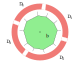
\includegraphics[width=5cm]{figs/consecDataStr}
\end{center}
\end{frame}

%\def\mitem{\medskip\item}
\def\fitem#1#2{\textcolor{hard}{\small (#1)}~~#2 \medskip \\}
\def\fpitem#1#2{\phantom{\small (#1)}~~#2 \medskip \\}

\begin{frame} \frametitle{Description of data structure}
\begin{definition}
	A cell is \emph{big} if it has size at least $N^{\frac14}$. Otherwise it is \emph{small}.
\end{definition} \bigskip \pause

\begin{center} \begin{tabular}{lcc}
\makecell[l]{
	\fitem{1}{Graph of VD in a form of adjacency list,}
	\fitem{2}{{\it Dynamic nearest neighbor} structure for sites,}
	\fitem{3}{Graph of big cells stored as adjacency list,}
	\fitem{4}{For each big cell:}
	\fpitem{4}{–~linked list of DCRs,}
	\fpitem{4}{–~binary search tree of vertices in circular order.}
} & \hspace{-0.95cm} &
	\makecell[c]{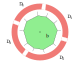
\includegraphics[width=4.5cm]{figs/consecDataStr}}
\end{tabular}
\end{center}
\end{frame}

\def\lrp#1{\left( #1 \right)}
\def\lrc#1{\left\lceil#1\right\rceil}
\def\otl{$\Ot(1)$ } \def\Ot{\tilde O}
\newcommand{\nof}{N^\frac{1}{4}}
\newcommand{\noh}{N^\frac{1}{2}}
\newcommand{\ntf}{N^\frac{3}{4}}

\begin{frame} \frametitle{Handling insertion}
\vspace{-7mm}
\begin{block}{\vspace*{-3ex}}
	Initialize queue; look at cells one-by-one, on each step add to it \\
	unprocessed cells with changes, then implement changes.
\end{block} \pause

\begin{itemize}
	\item Small cell: look at each paw to find neighboring cells needing changes, \\
	    add them to the queue.
	\mitem Big cell: ask DCRs to return Voronoi circles that enclose $s_N$, \\
	    add corresponding cells to the queue.
\end{itemize} \vspace{-2mm} \pause

\begin{block}{\vspace*{-3ex}} \vspace{-3.6mm}
{\small $$\text{Time complexity:\quad}
\Ot \lrp{
s\nof +
\sum_{i=1}^{|B|}  \lrp{ \lrc{\frac{|b_i|}{\nof }}+\ell_i}
+ \ntf + s\nof
}.
$$} \vspace{-2.6mm} \pause

\centerline{This is $\Ot(\ntf)$ amortized.}
\end{block}
\end{frame}

%\nfch{Ongoing research:}{\~Optimal-Time Incremental}{\Huge Voronoi Diagrams}

\begin{frame} \frametitle{Divide-and-conquer} \vspace{1.2mm}
Time complexity $\Ot(N^{\frac34})$ is not bad, but the lower bound is $N^{\frac12}$. Can we meet it? \\ \smallskip
The idea is to use divide-and-conquer approach. It can allow us to omit \\
doing unnecessary work. \bigskip

\begin{tabular}{lll}
\makecell[c]{
	\includegraphics[width=7.5cm]{figs/example}
} & \hspace{0.8cm} & \pause
\makecell[l]{
	\fitem{1}{Dividing line,}
	\fitem{2}{Beach lines,}
	\fitem{3}{Blue and red forests,}
	\fitem{4}{Merge curve.} \phantom{x} \\
}
\end{tabular}
\end{frame}

%\fch{Previous research:}{Polyhedra glued from regular pentagons}

\begin{frame}
\frametitle{Gluings}

\begin{definition}[{{\scriptsize Alexandrov 1950}}]
\label{def:razvertka}
	A {\itshape gluing} is a set of polygons equipped with
	a number of rules describing \\ the way
	edges of these polygons must be glued to each other.
\end{definition} \bigskip

\begin{figure}
	\centering
	\begin{subfigure}[m]{0.41\textwidth}
		\centering
		
\includegraphics[scale=1.12]{figs_pres/alex_example_1}
	\end{subfigure}
~
	\centering
	\begin{subfigure}[m]{0.48\textwidth}
		\centering
		
\includegraphics[scale=0.81]{figs_pres/alex_example_stefan_1}
	\end{subfigure}
\end{figure} \vspace{2.8mm}
\end{frame}

%%%%%%%%%%%%%%%%

\begin{frame}
\frametitle{Alexandrov's Theorem}

\vspace{3.8mm}

\begin{block}{Theorem ({\scriptsize Alexandrov 1950})}
	\itshape
	If a gluing is homeomorphic to a sphere and the sum of angles at each of its vertices is
	$\le 360^\circ$\!, there $\exists\,!$ convex polyhedron that corresponds to this gluing.
\end{block} \medskip

\begin{figure}
	\centering
	\begin{subfigure}[m]{0.46\textwidth}
		\centering
		\input{figs_pres/alex_example_2}
	\end{subfigure}
~
	\centering
	\begin{subfigure}[m]{0.46\textwidth}
		\centering
		\input{figs_pres/alex_example_stefan_2}
	\end{subfigure}
\end{figure}

\end{frame}

%%%%%%%%%%%%%%%%

\begin{frame} \frametitle{Polyhedron Reconstruction}

\textcolor{hard}{\bf The proof of Alexandrov's theorem is non-constructive.} \\
Each of the following problems is still open:

\smallskip

\begin{block}{Alexandrov's Problem} \small
	Given a gluing $\mathcal T$ satisfying the conditions of Alexandrov's Theorem, \\
	find the convex polyhedron corresponding to it.
\end{block}

\begin{block}{Cauchy Rigidity Problem ({\scriptsize \acite{DO07}, 23.22})} \small
	A {\itshape poly-time} algorithm that takes as input edge lengths of a triangulated
	convex polyhedron, and outputs approximate coordinates of its vertices.
\end{block}

\begin{block}{Skeleton Reconstruction Problem} \small
	A {\itshape poly-time} algorithm that, given a net satisfying the conditions of
	Alexandrov's Theorem, {\itshape finds the skeleton} of the
	convex polyhedron corresponding to it.
\end{block} \vspace{2.5mm}
\end{frame}

%%%%%%%%%%%%%%%%

\begin{frame} \frametitle{Edge-to-Edge Gluings of Regular Polygons}
\vspace{0.12cm}

Maybe Alexandrov's Problem becomes easier, if we start building the gluings \\
from similar simple blocks? \bigskip

\begin{definition}
	A gluing is {\itshape edge-to-edge} if every edge is glued to another entire edge.
\end{definition} \medskip

\begin{center}
	\includegraphics[width=11.4cm]{figs_pres/hex_glued} \\
	\acite{kl17-hex}
\end{center}
\end{frame}

%%%%%%%%%%%%%%%%

\begin{frame} \frametitle{Polyhedra glued from regular pentagons}
One can enumerate all gluings of pentagons. Here are all the polyhedra \\
    that can be obtained: \vspace{-1.2mm}

\begin{figure}
\centering
\begin{subfigure}[m]{0.15\columnwidth}
	\tikz{
	\filldraw[draw=edHr,thick,fill=fill1,fill opacity=0.55,rotate=34]
	(0:0.95cm) -- (72:0.95cm) -- (144:0.95cm) -- (216:0.95cm) -- (288:0.95cm) -- cycle;
}
\end{subfigure}
~~
\begin{subfigure}[m]{0.21\columnwidth}
	\def\fltn#1#2#3{(-0.85 * #1 cm + 1.2 * 0.7 * #3 cm + 0.5 * #2 cm,
	1.02 * #2 cm - 1.2 * 0.4 * #3 cm - 0.1 * #1 cm)}

\begin{center} \tikz[scale=1.4,rotate=25]{
\def\a{\fltn{0.7150286699726232}{0.0}{0.0} node{ }}
\def\b{\fltn{-0.31405294951344975}{0.8481487561449743}{-0.9163273343621601} node{ }}
\def\c{\fltn{-0.31405295029381125}{-0.8481662893257657}{0.9163111045353434} node{ }}
\def\d{\fltn{-0.16391141635587947}{-0.47693220123372715}{-0.0000091269006132692} node{ }}
\def\e{\fltn{-0.16391141696515857}{0.476932200185524}{0.0} node{ }}
\def\f{\fltn{-0.31405295029381125}{0.0}{0.0} node{ }}

\draw [color=thr] \a -- \e;
\draw [thick,color=edThr, dashed] \a -- \e;

\zal 1 \b -- \e -- \f -- \d -- \a -- cycle;
\zal 4 \e -- \c -- \a -- \d -- \f -- cycle;

\draw \a -- \b;
\draw \a -- \c;
\draw \b -- \f;
\draw \f -- \c;
\draw \b -- \d;
\draw \c -- \e;

\draw [thick,color=edHr] \c -- \d;
\draw [thick,color=edHr] \b -- \e -- \f -- \d -- \a;
} \end{center}
\end{subfigure}
~~
\begin{subfigure}[m]{0.25\columnwidth}
	\def\fltn#1#2#3{( #1 cm - 0.34 * #2 cm, #3 cm - 0.28* #2 cm)}

\begin{center} \tikz[scale=1.4]{
\def\a{\fltn{1.2935958265860046}{0.0}{0.0} node{ }}
\def\b{\fltn{0.9070763359531865}{-0.9222812387547359}{-0.00000000515911} node{ }}
\def\c{\fltn{-0.18790239082433305}{0.07874814457929721}{-0.6457420918350443} node{ }}
\def\d{\fltn{-0.18790239078823043}{0.07874814099060924}{0.6457420871720928} node{ }}
\def\e{\fltn{-1.1003360812768423}{0.4611406221034601}{-0.4999999973402255} node{ }}
\def\f{\fltn{-1.1003360812402079}{0.46114061650396965}{0.5000000026587861} node{ }}
\def\g{\fltn{0.43749429323987804}{0.5168076669346257}{0.0} node{ }}
\def\h{\fltn{-0.06168951174342411}{-0.6743039564170403}{-0.0000000037373} node{ }}

\draw [color=thr] \g -- \d;
\draw [color=thr] \g -- \f;
\draw [color=thr] \g -- \e;
\draw [color=thr] \g -- \c;
\draw [color=thr] \g -- \a;
\draw [color=thr] \a -- \d;

\draw [thick,color=edThr, dashed] \c -- \g -- \d;
\draw [thick,color=edThr, dashed] \g -- \a;

\zal 5 \b -- \h -- \d -- cycle;
\zal 3 \a -- \b -- \h -- \c -- cycle;
\zal 1 \f -- \d -- \h -- \c -- \e -- cycle;

\draw \d -- \b -- \a;
\draw \c -- \b -- \a -- cycle;
\draw \h -- \c -- \b -- cycle;
\draw \h -- \b -- \d -- cycle;
\draw \h -- \f -- \e -- cycle;
\draw \c -- \e -- \h -- cycle;
\draw \d -- \f -- \h -- cycle;

\draw [thick,color=edHr] \f -- \d -- \h -- \c -- \e -- cycle;
\draw [thick,color=edHr] \h -- \b -- \a;
} \end{center}
\end{subfigure}
~~
\begin{subfigure}[m]{0.28\columnwidth}
	\def\fltn#1#2#3{( 0.48 * 1.1 * #2 cm - 0.71 * 1.1 * #1 cm, 0.8 * #3 cm - 0.3 * #1 cm - 0.35 * #2 cm )}

\begin{center} \tikz[scale=1.5]{
\def\a{\fltn{1.1441186330689892}{0.0}{0.0} node{ }}
\def\b{\fltn{-0.00000096041478}{0.6605555441877259}{-0.9341722591401773} node{ }}
\def\c{\fltn{-1.1441193883103131}{-0.0000043143566}{-0.0000016231994} node{ }}
\def\d{\fltn{0.0000002051230056}{-0.660552576215044}{0.9341757852715699} node{ }}
\def\e{\fltn{0.3535525197824853}{-0.612376698215449}{0.000002436489} node{ }}
\def\f{\fltn{-0.35355132602086625}{-0.20413060947901404}{-0.577352984617954} node{ }}
\def\g{\fltn{0.35355410836555906}{0.612378749043792}{0.0} node{ }}
\def\h{\fltn{-0.35355291484900464}{0.204129462645888}{0.5773492685115242} node{ }}

\draw [color=thr] \d -- \e -- \f -- \c;
\draw [color=thr] \a -- \e;
\draw [color=thr] \f -- \b;

\draw [thick,color=edThr, dashed] \d -- \e -- \f -- \c;
\draw [thick,color=edThr, dashed] \a -- \e;
\draw [thick,color=edThr, dashed] \f -- \b;

\zal 2 \d -- \h -- \g -- \a -- cycle;
\zal 6 \d -- \h -- \c -- cycle;
\zal 1 \c -- \h -- \g -- \b -- cycle;
\zal 5 \a -- \g -- \b -- cycle;

\draw \a -- \b -- \c -- \d -- cycle;

\draw [thick,color=edHr] \d -- \h -- \g -- \a;
\draw [thick,color=edHr] \c -- \h;
\draw [thick,color=edHr] \g -- \b;
} \end{center}
\end{subfigure}
\end{figure}

\vspace{-8.5mm}

\begin{figure}
\centering
\hspace{-8mm}
\begin{subfigure}[m]{0.235\columnwidth}
	\def\fltn#1#2#3{(#1 cm + 0.44 * #3 cm, #2 cm + 0.22 * #3 cm)}

\begin{center} \tikz[scale=1.2,rotate=120]{
\def\a{\fltn{1.1441197647858687}{0.0}{0.0} node{ }}
\def\b{\fltn{-0.35355163051439026}{0.2041215106112333}{-0.5773524759670514} node{ }}
\def\c{\fltn{-1.8512230326059445}{-0.40825211084630797}{-0.5773526337782059} node{ }}
\def\d{\fltn{-0.3535516373056661}{-0.6123736214577439}{-0.00000015778708221} node{ }}
\def\e{\fltn{1.8512225918511154}{0.408252018329011}{0.577352475975189} node{ }}
\def\f{\fltn{0.35355119655087724}{0.6123735289175027}{0.0} node{ }}
\def\g{\fltn{-1.1441202055378052}{-0.000000092541959995}{-0.000000157789119} node{ }}
\def\h{\fltn{0.353551189759604}{-0.2041216031515996}{0.5773523181800547} node{ }}

\draw [color=thr] \h -- \d -- \a -- cycle;
\draw [color=thr] \h -- \e -- \f -- cycle;
% \draw [color=thr, dashed] \h -- \f -- \g -- cycle;
\draw [color=thr] \d -- \h -- \g -- cycle;
\draw [color=thr] \a -- \e -- \h -- cycle;
% \draw [color=thr, dashed] \g -- \c -- \d -- cycle;

\draw [thick,color=edThr, dashed]  \a -- \h -- \d;
\draw [thick,color=edThr, dashed] \g -- \d;
\draw [thick,color=edThr, dashed] \h -- \f;

\zal 1 \a -- \f -- \b -- \d -- cycle;
\zal 4 \d -- \b -- \g -- \c -- cycle;
\zal 5 \g -- \b -- \f -- cycle;
\zal 3 \f -- \a -- \e -- cycle;

\draw \d -- \a -- \b -- cycle;
\draw \f -- \a -- \b -- cycle;
\draw \d -- \b -- \c -- cycle;
\draw \g -- \b -- \c -- cycle;
\draw \a -- \e -- \f -- cycle;
\draw \b -- \f -- \g -- cycle;

\draw [thick,color=edHr] \d -- \b -- \f -- \a -- \e;
\draw [thick,color=edHr] \c -- \g -- \b;
}\end{center}
\end{subfigure}
~~
\begin{subfigure}[m]{0.22\columnwidth}
\centering
	\def\fltn#1#2#3{( #1 cm - 0.38 * #2 cm, #3 cm - 0.2 * #2 cm)}

\begin{center} \tikz[scale=1.28]{
\def\a{\fltn{1.4310957967719642}{0.0}{0.0} node{ }}
\def\b{\fltn{0.7162308035620336}{0.3787815383028905}{-0.587786175174265} node{ }}
\def\c{\fltn{-0.7155478984982786}{0.00000000009007338}{-1.2393653153906468} node{ }}
\def\d{\fltn{-0.8671531615396659}{0.3787815383070919}{-0.3263809830922096} node{ }}
\def\e{\fltn{-0.7155478985611488}{-0.0000000003687175}{1.2393653153533593} node{ }}
\def\f{\fltn{0.15092235791116757}{0.3787815381579165}{0.9141671585035448} node{ }}
\def\g{\fltn{-0.0000000000001461}{0.7549741064176964}{0.0} node{ }}
\def\h{\fltn{0.15092235791177575}{-0.3787815383030031}{-0.9141671584442804} node{ }}
\def\i{\fltn{-0.8671531614092768}{-0.37878153847290486}{0.32638098324776055} node{ }}
\def\j{\fltn{0.7162308035616037}{-0.37878153839618434}{0.5877861751136217} node{ }}
\def\k{\fltn{-0.0000000000001931}{-0.7549741069521263}{0.000000000221224} node{ }}

\draw [color=thr] \g -- \a -- \b -- cycle;
\draw [color=thr]\g -- \b -- \c -- cycle;
\draw [color=thr] \g -- \d -- \e -- cycle;
\draw [color=thr] \g -- \c -- \d -- cycle;
\draw [color=thr] \g -- \e -- \f -- cycle;
\draw [color=thr] \g -- \a -- \f -- cycle;
\draw [color=thr] \j -- \e -- \f -- cycle;
\draw [color=thr] \j -- \a -- \f -- cycle;
\draw [color=thr] \h -- \c -- \b -- cycle;

\draw [thick,color=edThr, dashed] \j -- \f -- \g -- \b;
\draw [thick,color=edThr, dashed] \e -- \f;
\draw [thick,color=edThr, dashed] \g -- \d;
\draw [thick,color=edThr, dashed] \b -- \h;

\zal 1 \c -- \d -- \i -- \k -- \h -- cycle;
\zal 2 \b -- \h -- \k -- \j -- \a -- cycle;
\zal 4 \j -- \k -- \i -- \e -- cycle;
\zal 3 \e -- \i -- \d -- cycle;

\draw \h -- \b -- \a -- cycle;
\draw \i -- \d -- \c -- cycle;
\draw \i -- \e -- \d -- cycle;
\draw \k -- \h -- \a -- cycle;
\draw \k -- \c -- \h -- cycle;
\draw \k -- \i -- \c -- cycle;
\draw \k -- \e -- \i -- cycle;
\draw \k -- \j -- \e -- cycle;
\draw \k -- \a -- \j -- cycle;

\draw [thick,color=edHr] \e -- \i -- \k -- \j;
\draw [thick,color=edHr] \a -- \j -- \k -- \h -- \b -- cycle;
\draw [thick,color=edHr] \h -- \c -- \d -- \i -- \k -- cycle;
} \end{center}
\end{subfigure}
~~
\begin{subfigure}[m]{0.19\columnwidth}
	\def\fltn#1#2#3{( 0.95 * #1 cm + 1.3 * 0.48 * #3 cm, 0.95 * #2 cm + 1.3 * 0.26 * #3 cm - 0.08 * #1 cm)}

\begin{center} \tikz[rotate=75,scale=1.4]{
\def\a{\fltn{1.7964059390811467}{0.0}{0.0} node{ }}
\def\b{\fltn{1.0741858668825588}{0.3774601538724013}{0.5795877841641639} node{ }}
\def\c{\fltn{0.4627696824462514}{-0.37047892722529857}{0.8379622805377634} node{ }}
\def\d{\fltn{0.4627696824462251}{-0.9162070816198993}{-0.000000000674378481} node{ }}
\def\e{\fltn{1.0741858668825224}{-0.3774601544164369}{-0.5795877838098117} node{ }}
\def\f{\fltn{0.46276968244613376}{0.37047892643871677}{-0.8379622808853392} node{ }}
\def\g{\fltn{0.4627696824461601}{0.9162070813351211}{0.0} node{ }}
\def\h{\fltn{-1.796405938942955}{0.0000000000684636823}{-0.00000000034584134394} node{ }}
\def\i{\fltn{-1.0741858671205824}{-0.579587784025112}{0.3774601534086557} node{ }}
\def\j{\fltn{-0.46276968266375634}{-0.0000000009484149785}{0.9162070812362096} node{ }}
\def\k{\fltn{-0.4627696822356244}{0.8379622786720125}{0.3704789273536469} node{ }}
\def\l{\fltn{-1.0741858665333857}{0.5795877843576744}{-0.3774601545686791} node{ }}
\def\m{\fltn{-0.4627696825916457}{-0.8379622802654594}{-0.3704789276593546} node{ }}
\def\n{\fltn{-0.462769682167164}{0.0000000011376730667}{-0.9162070817606903} node{ }}

\draw [color=thr] \a -- \c;
\draw [color=thr] \b -- \j;
\draw [color=thr] \b -- \k;
\draw [color=thr] \c -- \i;
\draw [color=thr] \d -- \i;
\draw [color=thr] \h -- \j;
\draw [color=thr] \h -- \k;

\draw [color=thr] \b -- \c;
\draw [color=thr] \c -- \d;
\draw [color=thr] \c -- \j;
\draw [color=thr] \i -- \j;
\draw [color=thr] \j -- \k;
\draw [color=thr] \i -- \m;
\draw [color=thr] \h -- \i;

\draw [thick,color=edThr, dashed] \b -- \c;
\draw [thick,color=edThr, dashed] \c -- \d;
\draw [thick,color=edThr, dashed] \c -- \j;
\draw [thick,color=edThr, dashed] \i -- \j;
\draw [thick,color=edThr, dashed] \j -- \k;
\draw [thick,color=edThr, dashed] \i -- \m;
\draw [thick,color=edThr, dashed] \h -- \i;

\zal 4 \a -- \b -- \g -- \f -- \e -- cycle;
\zal 3 \h -- \l -- \n -- \m -- cycle;
\zal 6 \d -- \e -- \a -- cycle;
\zal 1 \m -- \n -- \f -- \e -- \d -- cycle;
\zal 2 \k -- \g -- \f -- \n -- \l -- cycle;

\draw \a -- \g;
\draw \a -- \f;
\draw \a -- \d;
\draw \e -- \m;
\draw \e -- \n;
\draw \g -- \l;
\draw \f -- \l;
\draw \h -- \n;
\draw \h -- \m;

\draw [thick,color=edHr] \a -- \b;
\draw [thick,color=edHr] \a -- \e;
\draw [thick,color=edHr] \b -- \g;
\draw [thick,color=edHr] \d -- \e;
\draw [thick,color=edHr] \d -- \m;
\draw [thick,color=edHr] \e -- \f;
\draw [thick,color=edHr] \f -- \g;
\draw [thick,color=edHr] \f -- \n;
\draw [thick,color=edHr] \g -- \k;
\draw [thick,color=edHr] \h -- \l;
\draw [thick,color=edHr] \k -- \l;
\draw [thick,color=edHr] \l -- \n;
\draw [thick,color=edHr] \m -- \n;

} \end{center}
\end{subfigure}
~~
\begin{subfigure}[m]{0.18\columnwidth}
\tikz[scale=0.69]{
	\def\fl#1#2#3{(0.94868 * #1 cm + 0.56 * 1.2 * #2 cm,
	-0.42 * 0.72 * #1 cm + 0.6 * 0.72 * 1.2 * #2 cm + 1.05 * #3 cm)}
\def\zl#1{\filldraw[thick , color=edHr , fill=fill#1 , fill opacity = 0.55] }
\def\g{1.618034}
\def\gg{0.618034}

\def\AA{\fl{0}{\g}{\gg}}
\def\AB{\fl{0}{\g}{-1 * \gg}}
\def\AC{\fl{0}{-1 * \g}{\gg}}
\def\AD{\fl{0}{-1 * \g}{-1 * \gg}}

\def\BA{\fl{\g}{\gg}{0}}
\def\BB{\fl{\g}{-1 * \gg}{0}}
\def\BC{\fl{-1 * \g}{\gg}{0}}
\def\BD{\fl{-1 * \g}{-1 * \gg}{0}}

\def\CA{\fl{\gg}{0}{\g}}
\def\CB{\fl{-1 * \gg}{0}{\g}}
\def\CC{\fl{\gg}{0}{-1 * \g}}
\def\CD{\fl{-1 * \gg}{0}{-1 * \g}}

\def\UTR{\fl{1}{1}{1}}
\def\UTL{\fl{-1}{1}{1}}
\def\UBR{\fl{1}{-1}{1}}
\def\UBL{\fl{-1}{-1}{1}}

\def\DTR{\fl{1}{1}{-1}}
\def\DTL{\fl{-1}{1}{-1}}
\def\DBR{\fl{1}{-1}{-1}}
\def\DBL{\fl{-1}{-1}{-1}}

\draw[color=thr] \BA -- \UTR -- \AA -- \AB -- \DTR -- cycle;
\draw[color=thr] \AA -- \AB -- \DTL -- \BC -- \UTL -- cycle;

\draw[color=thr] \BC -- \BD -- \DBL -- \CD -- \DTL -- cycle;
\draw[color=thr] \BD -- \BC -- \UTL -- \CB -- \UBL -- cycle;

\draw[color=thr] \CC -- \CD -- \DTL -- \AB -- \DTR -- cycle;
\draw[color=thr] \CC -- \CD -- \DBL -- \AD -- \DBR -- cycle;

\draw[thick,color=edThr,dashed] \UTL -- \BC -- \BD;
\draw[thick,color=edThr,dashed] \AA -- \AB -- \DTR;
\draw[thick,color=edThr,dashed] \BC -- \DTL -- \AB;
\draw[thick,color=edThr,dashed] \DTL -- \CD;
\draw[thick,color=edThr,dashed] \DBL -- \CD -- \CC;

\zl 4 \AC -- \AD -- \DBR -- \BB -- \UBR -- cycle;
\zl 6 \AC -- \AD -- \DBL -- \BD -- \UBL -- cycle;

\zl 1 \BB -- \BA -- \UTR -- \CA -- \UBR -- cycle;
\zl 2 \BA -- \BB -- \DBR -- \CC -- \DTR -- cycle;

\zl 3 \CB -- \CA -- \UBR -- \AC -- \UBL -- cycle;
\zl 5 \CB -- \UTL -- \AA -- \UTR -- \CA -- \CB;
}
\end{subfigure}
\end{figure} \vspace{2mm}
\end{frame}

\renewcommand{\thefootnote}{*}

\def\P{\mathcal P}
\def\ball#1{B_r ( #1 )}

\begin{frame}
\frametitle{Precision of vertex location based on the approximation}
\vspace{0.8mm}

\begin{theorem}
	If $\mathcal D \gamma < \pi / 2$, then each vertex of $\P$ lies within an $r$-ball centered at the \\
	corresponding vertex of $P$, where
	\centerline{$r = E^2 \cdot  L \cdot 2 \sin ( \mathcal D \gamma / 2 ) + E \mu$.}
\end{theorem} \smallskip

	$\P$ — convex polyhedron corresponding to a given net, \\
	$P$ — approximation of $\P$. $\mathcal D$ — $\max$ degree of a vertex of $P$. \\
	$\mu$ — $\max$ edge discrepancy between $P$ and $\P$, \\
	$\gamma$ — $\max$ face angle discrepancy. \\

\begin{figure}
	\centering
	\begin{subfigure}[b]{0.37\columnwidth}
		\centering
		\includegraphics[scale=0.86]{figs_pres/anglePathOffset}
	\end{subfigure}
~
	\begin{subfigure}[b]{0.37\columnwidth}
		\centering
		\includegraphics[scale=0.86]{figs_pres/edgePathOffset}
	\end{subfigure}
\end{figure}
\end{frame}

%%%%%%%%%%%%%%%%

\begin{frame}
\frametitle{Determining the shape from the gluing}

\begin{tabular}{lll}
\makecell[l]{
	Let $pqr$, $sqr$ be adjacent faces of $P$. \\
	\textcolor{hard}{\bf Are there edges $ps$, $qr$ in $\P$?} \bigskip \\
	Assume $pqr$ is not vertical and $P$ lies {\itshape below it}. \\
	Consider three planes $\Pi_1$, $\Pi_2$, $\Pi_3$ tangent \\
	to $\ball{p}$, $\ball{q}$, $\ball{r}$.
}
& \hspace{0.47cm} & \hspace{-3.2cm}
	\def\scopescale{0.51}
	\makecell[c]{\definecolor{ploskost}{RGB}{96,214,232}
\definecolor{sharik}{RGB}{181,56,43}

\def\flatn#1#2#3{(0.94868 * #1 cm + 0.4 * #2 cm,
	-0.31623 * #1 cm + 0.533333 * #2 cm + #3 cm)}
\def\punktir{\draw[dashed,color=hr]}
\def\thekrug#1{
	\filldraw #1 circle[radius=0.34mm];
	\filldraw[fill=sharik,fill opacity=0.72,draw=black] #1 circle [radius=0.5cm]}

\def\zleft{0.883883}
\def\zright{-1.767767}
\def\zz{-0.53033}

\def\pcenter{\flatn{-3}{0.5}{0}}
\def\ptangent{\flatn{-2.83333}{0.5}{0.471405}}

\def\qcenter{\flatn{0}{-2}{0}}
\def\qtangent{\flatn{-0.166667}{-2}{-0.471405}}

\def\rcenter{\flatn{0}{2}{0}}
\def\rtangent{\flatn{-0.166667}{2}{-0.471405}}

\def\sacenter{\flatn{2.5}{-0.5}{-2.3}}
\def\sbcenter{\flatn{2.5}{-0.5}{-0.65}}

\def\stransition{\flatn{2.5}{-0.5}{-1.41421}}
\def\sproj{\flatn{2.5}{-0.5}{0}}

\tikz{ \begin{scope}[scale=\scopescale]
% Кружок вершины p и то, что его обслуживает
	\punktir \ptangent -- \pcenter -- \flatn{-2.5}{0.5}{0};
	\punktir \pcenter -- \flatn{-3}{0}{0};
	\thekrug{\pcenter};
	\punktir \flatn{-2.5}{0.5}{0} -- \flatn{-1.5}{0.5}{0};
	\draw[thick] \flatn{-4}{0}{0} -- \flatn{-1.5}{0}{0};
%%

% Кружок вершины s_1 и то, что его обслуживает
	\punktir \flatn{2.5}{-0.5}{-1.8} -- \sacenter;
	\thekrug{\sacenter};
	\punktir \flatn{2.5}{-0.5}{-1.8} -- \stransition;
%%

% Та самая плоскость
	\filldraw[fill=ploskost,draw=ploskost, fill opacity=0.75]
		\flatn{-4}{3.075}{\zleft} -- \flatn{-4}{-3.075}{\zleft} --
		\flatn{3.5}{-3.075}{\zright} -- \flatn{3.5}{3.075}{\zright};
%%

% Несколько линий от точек касания
	\filldraw[fill=hr,draw=hr] \ptangent circle[radius=0.34mm];
	\punktir \ptangent -- \flatn{-1.5}{0.5}{0};
	\filldraw[fill=hr,draw=hr] \qtangent circle[radius=0.34mm];
	\punktir \qtangent -- \qcenter;
	\filldraw[fill=hr,draw=hr] \rtangent circle[radius=0.34mm];
	\punktir \rtangent -- \rcenter;
%%

% Кружок вершины s_2 и то, что его обслуживает
	\filldraw[fill=hr,draw=hr] \stransition circle[radius=0.34mm];
	\punktir \flatn{2.5}{-0.5}{-0.15} -- \stransition;
	\thekrug{\sbcenter};
	\punktir \flatn{2.5}{-0.5}{-0.15} -- \sproj;
	\punktir \flatn{0}{-0.5}{0} -- \sproj -- \flatn{2.5}{0}{0};
%%

% Два шарика на оси y
	\draw [thick,->] \flatn{0}{1.5}{0} -- \flatn{0}{3.75}{0};
	\thekrug{\rcenter};
	\draw [thick] \flatn{0}{-2.5}{0} -- \flatn{0}{1.5}{0};
	\thekrug{\qcenter};
	\draw [thick] \flatn{0}{-3.75}{0} -- \flatn{0}{-2.5}{0};
%%

% Линии, висящие в воздухе
	\punktir \flatn{-1.5}{0.5}{0} -- \flatn{0}{0.5}{0};
	\draw [thick,->] \flatn{-1.5}{0}{0} -- \flatn{4}{0}{0};
%%

% Подписи узлов
	\draw \pcenter node[left]{\footnotesize $p$};
	\draw \qcenter node[right]{\footnotesize\ \,$q$};
	\draw \rcenter node[right]{\footnotesize\ \ $r$};
	\draw \sacenter node[right]{\footnotesize $s_1$};
	\draw \sbcenter node[right]{\footnotesize\ \ $s_2$};
	\draw \stransition node[right]{\footnotesize $t$};
%%
\end{scope} }}
\end{tabular}

\begin{theorem}
	If $s$ lies below $\Pi_1$, $\Pi_2$ and $\Pi_3$ and the distance from $s$ to each of the planes \\
	$\Pi_1$, $\Pi_2$ and $\Pi_3$ is greater than $r$, then the edge $qr$ must be in $\P$.
\end{theorem} \medskip

\textcolor{hard}{\bf Implemented on {\itshape Haskell.}} \\
Geometric methods can also be used.
\vspace{2mm}
\end{frame}

\def\fitem#1#2{\textcolor{hard}{\small (#1)}~~#2 \medskip \\}

\begin{frame}
\frametitle{Conclusion}

\begin{center} \begin{tabular}{lll}
\multicolumn{3}{l}{\textcolor{hard}{\bf Results achieved: \medskip}} \\
\makecell[l]{\fitem{1}{Full list of the polyhedra that are made by edge-to-edge \\
	gluings of regular pentagons}} & &
\makecell[c]{GRAPHICS} \\
\makecell[l]{\fitem{2}{First sublinear algorithm for maintaining \\
	the graph of a Voronoi diagram}} & &
\makecell[c]{GRAPHICS} \\
\multicolumn{3}{l}{\textcolor{hard}{\bf Ongoing research: \medskip}} \\
\makecell[l]{\fitem{3}{Algorithm for maintaining the graph \\
	of a Voronoi Diagram with the optimal time complexity}} & &
\makecell[c]{GRAPHICS}
\end{tabular} \end{center} \smallskip

\hrule \vspace{0.26cm}
\begin{center}
	{\LARGE Thank you for your attention!}
\end{center} \vspace{1.2mm}
\end{frame}

\begin{frame}
\scriptsize
	\bibliography{zba_ths,rg}
	\bibliographystyle{apalike}
\end{frame}

\end{document}